% The standing setup of the Frobenius chapter: K/ℚ Galois, 𝒪_K/ℤ,
% a prime 𝔭 above (p), and the residue tower 𝒪_K/𝔭 ≅ 𝔽_{p^f} over 𝔽_p.
% Source: book/tex/alg-NT/frobenius.tex (chapter opening) — tikzcd.
\documentclass[border=2mm]{standalone}
\usepackage{tikz}
\usepackage{amssymb}
\usepackage{amsmath}
\begin{document}
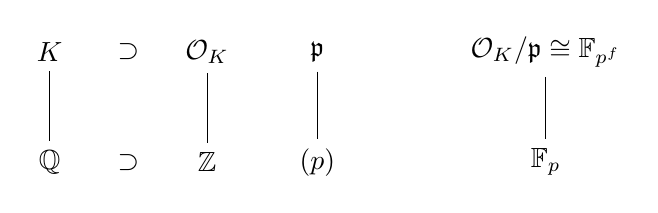
\begin{tikzpicture}
  \node (K)  at (0,1.4)   {$K$};
  \node (Q)  at (0,0)     {$\mathbb{Q}$};
  \node (s1) at (1.0,1.4) {$\supset$};
  \node (s2) at (1.0,0)   {$\supset$};
  \node (OK) at (2.0,1.4) {$\mathcal{O}_K$};
  \node (Z)  at (2.0,0)   {$\mathbb{Z}$};
  \node (pp) at (3.4,1.4) {$\mathfrak{p}$};
  \node (p)  at (3.4,0)   {$(p)$};
  \node (F1) at (6.3,1.4) {$\mathcal{O}_K/\mathfrak{p} \cong \mathbb{F}_{p^f}$};
  \node (F2) at (6.3,0)   {$\mathbb{F}_p$};
  \draw (K) -- (Q);
  \draw (OK) -- (Z);
  \draw (pp) -- (p);
  \draw (F1) -- (F2);
\end{tikzpicture}
\end{document}
